% Tikz File 'decision_tree.tex'
\documentclass{standalone}
\usepackage{tikz}
\usetikzlibrary{positioning}
\newdimen\nodeDist
\nodeDist=20mm

\begin{document}

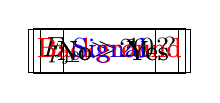
\begin{tikzpicture}[node/.style={draw, rectangle}]

  \node [node] (A) {$p_\perp > \SI{20}{\GeV}$ ?};
  
  \path (A) ++(-135:\nodeDist) node [node] (B) {\textcolor{red}{Background}};
  \path (A) ++(- 45:\nodeDist) node [node] (C) {$E_\mathrm{jet} > \SI{10}{\GeV}$ ?};
  \path (C) ++(-135:\nodeDist) node [node] (D) {\textcolor{red}{Background}};
  \path (C) ++(- 45:\nodeDist) node [node] (E) {\textcolor{blue}{Signal}};

  \draw (A) -- (B) node [left=0.1cm, pos=0.5] {No}(A);
  \draw (A) -- (C) node [right=0.1cm,pos=0.5] {Yes}(A);
  \draw (C) -- (D) node [left=0.1cm, pos=0.5] {No}(A);
  \draw (C) -- (E) node [right=0.1cm,pos=0.5] {Yes}(A);
\end{tikzpicture}

\end{document}

